\documentclass[12pt]{extarticle}
\linespread{1.5}

\title{Численные методы. ДЗ 15. Архитектура системы}
\author{Владимир Попов}
\date{\today}

\usepackage{cmap}
\usepackage[T2A]{fontenc}
\usepackage[english, russian]{babel}
\usepackage[utf8]{inputenc}
\usepackage{mathtools}
\usepackage{amsfonts}
\usepackage{graphicx}
\usepackage{listings}
\usepackage{courier}
\usepackage{indentfirst}
\usepackage{stmaryrd}
\usepackage{caption}
\captionsetup[figure]{labelformat=empty}

\usepackage{tikz}
\usepackage{tzplot}
\usetikzlibrary{arrows,decorations.pathmorphing,backgrounds,positioning,fit,petri}
\usetikzlibrary{calc,intersections,through,backgrounds, quotes, angles}
\usetikzlibrary{arrows,automata,positioning}
\tikzset{snake it/.style={decorate, decoration=snake}}
\usepackage{pgfplots,pgf-pie}

\usepackage{geometry} % Меняем поля страницы
\geometry{left=2cm}% левое поле
\geometry{right=1.5cm}% правое поле
\geometry{top=1cm}% верхнее поле
\geometry{bottom=2cm}% нижнее поле

\newtheorem{definition}{Определение}
\newtheorem{remark}{Ремарка!}
\newtheorem{theorem}{Теорема}

\newcommand{\implyarrow}{%
  \mathrel{\raisebox{1.3ex}{\rotatebox[origin=c]{90}{\mathhexbox37F}}}}

\DeclareMathOperator{\arccot}{arccot}

\usepackage{listings}
\usepackage{xcolor}

%New colors defined below
\definecolor{codegreen}{rgb}{0,0.6,0}
\definecolor{codegray}{rgb}{0.5,0.5,0.5}
\definecolor{codepurple}{rgb}{0.58,0,0.82}
\definecolor{backcolour}{rgb}{0.95,0.95,0.92}

%Code listing style named "mystyle"
\lstdefinestyle{mystyle}{
  backgroundcolor=\color{backcolour},   
  commentstyle=\color{codegreen},
  keywordstyle=\color{magenta},
  numberstyle=\tiny\color{codegray},
  stringstyle=\color{codepurple},
  basicstyle=\ttfamily\footnotesize,
  breakatwhitespace=false,         
  breaklines=true,                 
  captionpos=b,                    
  keepspaces=true,                 
  numbers=left,                    
  numbersep=5pt,                  
  showspaces=false,                
  showstringspaces=false,
  showtabs=false,                  
  tabsize=2
}

%"mystyle" code listing set
\lstset{style=mystyle}

\begin{document}

\begin{center}
    \Large\textbf{Архитектурное описание библиотеки количественного финансового анализа (QuantLib)}\\
    \vspace{0.5cm}
    \large\textit{Целевая аудитория: Разработчики}
\end{center}

\section{Контекст и назначение системы}
Разрабатываемая система представляет собой высокопроизводительную библиотеку для численного моделирования финансовых процессов (в частности, ценообразования опционов по модели Блэка-Шоулса).

\section{Структура системы}
Архитектура построена на основе \textbf{Layered style}. 

\begin{figure}[h!]
    \centering
    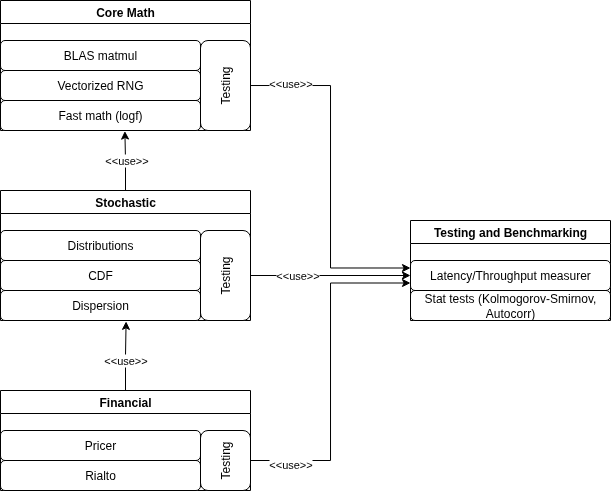
\includegraphics[width=0.8\textwidth]{scheme.png}
    \caption{Диаграмма пакетов разрабатываемой системы}
\end{figure}

Система декомпозирована на следующие модули:
\begin{itemize}
    \item \textbf{Core Math (C/C++, SIMD):} Слой платформозависимых оптимизаций. Содержит векторизованный (AVX-512) генератор \texttt{MinstdRandVec}, оптимизированное перемножение матриц с учетом кэш-локальности и кастомную функцию \texttt{logf} с точностью 3ULP.
    \item \textbf{Stochastic (C++):} Алгоритмический слой. Предоставляет генераторы из различных распределений (Normal, Gamma, ChiSquare), функции CDF и устойчивые к потере точности алгоритмы расчета дисперсии (\texttt{Disp1Pass}, \texttt{Disp2Pass}).
    \item \textbf{Financial (C++):} Бизнес-логика. Реализует прайсинг опционов (модули \texttt{Rialto} и \texttt{Pricer}) аналитическим методом и методом Монте-Карло с поддержкой пакетной обработки.
    \item \textbf{Testing and Benchmarking:} Содержит статистические тесты (Колмогорова-Смирнова, автокорреляция) и фреймворк \texttt{Runner} для замеров latency и throughput через \texttt{rdtscp} с защитой от out-of-order execution.
\end{itemize}

\section{Обоснование архитектурных решений}

\subsection{Разделение на вычислительное ядро и бизнес-логику:}
Финансовые модули изолированы от деталей работы с SIMD-инструкциями и аппаратными таймерами. Это позволяет разработчикам бизнес-логики оперировать высокоуровневыми концепциями, в то время как Core-разработчики могут менять реализацию \texttt{matmul} или RNG без влияния на верхний слой.

\subsection{Использование C для ядра и C++ для верхних уровней:}
Низкоуровневые вычисления реализованы на C с использованием \texttt{restrict} указателей для максимизации агрессивных оптимизаций компилятора. Статистический слой использует шаблоны C++ для обеспечения zero-cost абстракций над числами с плавающей точкой.

\subsection{Внедрение независимого инфраструктурного слоя Benchmarking:}
Система имеет критические нефункциональные требования к производительности. Поэтому профилирование вынесено в отдельный архитектурный компонент. Использование \texttt{taskset}, изоляции ядер и cpupower governor на уровне Makefile гарантирует, что разработчики будут получать воспроизводимые метрики, валидируя дизайн-требования к latency и throughput.


\end{document}